\chapter{Introductie}

\section{Probleemschets}

Het probleem dat in deze masterproef zal worden onderzocht doet zich heel specifiek voor bij verschillende experimenten die aan het IPEM worden uitgevoerd. Dit is de onderzoeksinstelling van het departement musicologie aan Universiteit Gent. De focus van het IPEM ligt vooral op onderzoek naar de interactie van muziek op fysieke aspecten van de mens zoals dansen, sporten en fysieke revalidatie. \cite{ipem2016}

Om de relatie tussen muziek en beweging te onderzoeken worden er tal van experimenten uitgevoerd. Deze experimenten maken gebruik van allerhande sensoren om bepaalde gebeurtenissen om te zetten in analyseerbare data. 

Bij een klassieke experiment wordt onderzocht wat de invloed is van muziek op de lichamelijke activiteit van een persoon. Alle bewegingen worden geregistreerd met een videocamera en verschillende sensoren.

Hierbij moeten minstens drie datastreams worden geanalyseerd: de videobeelden, de data van de accelerometer(s) en de afgespeelde audio. Een  uitdaging hierbij is de synchronisatie van deze verschillende datastreams. Om een goede analyse mogelijk te maken is het zeer gewenst dat men exact weet (tot op de milliseconde nauwkeurig) wanneer een bepaalde gebeurtenis in een datastream zich heeft voorgedaan, zodat men deze gebeurtenis kan vergelijken met de gebeurtenissen in de andere datastreams. Door de verschillen in samplefrequentie en door de latencies van elke opname is dit zeker geen sinecure. \cite{six2015multimodal}

Bij het IPEM maakt men gebruik van een systeem waarbij audio opnames het synchronisatieproces vereenvoudigen. Het principe werkt als volgt: men zorgt ervoor dat elke datastream vergezeld van een perfect gesynchroniseerde audiostream, afkomstig van een opname van het omgevingsgeluid. In het voorgaande experiment is dit eenvoudig te verwezenlijken. Bij de videobeelden kan automatisch een audiospoor mee worden opgenomen. De accelerometer kan geplaatst worden op een microcontroller vergezeld van een kleine microfoon.. Aangezien beide componenten zo dicht op de hardware geplaatst zijn is de latency tussen beide datastromen te verwaarlozen.\footnote{De latency van de audioverwerking op een \textit{Axoloti} microcontroller is vastgesteld op 0.333 ms. Meer informatie: \url{http://www.axoloti.com/more-info/latency/}} De afgespeelde audio kan gebruikt worden als referentie, aangezien dit uiteraard al een perfecte weergave is van het omgevingsgeluid. 

Na het uitvoeren van het experiment beschikt men dus over de gegevens van drie datastreams, waarbij er aan elke datastream een quasi perfect synchrone opname van het omgevingsgeluid is gekoppeld. Aangezien het experiment in één ruimte is uitgevoerd zijn de verschillende opnames van het omgevingsgeluid zeer gelijkend. Het probleem van de synchronisatie van de verschillende datastromen kan bijgevolg gereduceerd worden tot het synchroniseren van de verschillende audiostromen.

Door de typisch eigenschappen van geluid is het niet zo moeilijk om verschillende audiostromen te synchroniseren. Bij het IPEM heeft men een systeem ontwikkeld dat in staat is om verschillende audiostreams te synchroniseren.

Dit systeem heeft in de praktijk echter heel wat beperkingen. De grootste beperking is dat het synchronisatieproces pas kan worden uitgevoerd wanneer het experiment is afgelopen, en dit volledig handmatig. De opgenomen audiobestanden moet worden verzameld op een computer, vervolgens kan met behulp van de audiobestanden de latency van elke datastream worden berekend. Vervolgens kunnen de datastreams worden gesynchroniseerd. Voor de musicologen die deze experimenten uitvoeren is deze werkwijze veel te omslachtig. Daarom is een eenvoudiger realtime systeem om de synchronisatie uit te voeren zeer gewenst.

\begin{figure}[!h]
	\captionsetup{width=0.7\textwidth}
	\centering
	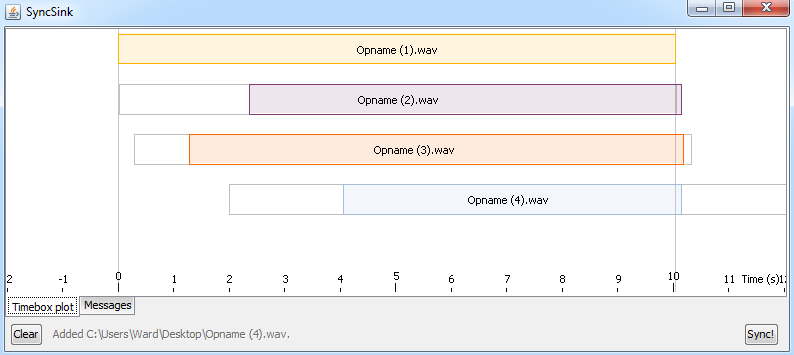
\includegraphics[width=0.5\textwidth]{syncsinc.png}
	\caption[Huidge werkwijze voor streamsynchronisatie]{Huidige werkwijze om streams te synchroniseren: Een drag and drop interface waarin de opgenomen fragmenten gesleept kunnen worden na afloop van het experiment. Vervolgens wordt de latency berekend.}
\end{figure}


Een ander probleem is iets vager en minder duidelijk te omschrijven. De resultaten van het kruiscovariantie algoritme bevatten soms afwijkingen die moeilijk te verklaren zijn. De precieze oorzaak hiervan, en hoe dit kan worden opgelost zal ook worden onderzocht. Ook is het kruiscovariantie algoritme in vergelijking met het accoustic fingerprinting algoritme véél gevoeliger voor storingen en ruis, veroorzaakt door slechte opnames. Aangezien de opnameapparatuur (zeker op microcontrollers) bij de uit te voeren experimenten vaak van slechte kwaliteit is, is het belangrijk om de algoritmes voldoende robuust te maken zodat ze hier niet over struikelen.

\section{Digitale audio}

Het vervolg van deze scriptie onderstelt dat de lezer een basiskennis heeft inzake digitale audio. In deze inleiding worden de belangrijkste zaken hieromtrent uitgelegd.

Om geluidsgolven digitaal te kunnen verwerken moeten ze worden geconverteerd naar reeksen van discrete waarden. Deze omzetting gebeurt met een ADC: een analog-to-digital converter. De meeste ADC's maken gebruik van de PCM (pulse-code modulation) voorstelling van audio. Bij PCM wordt het analoge signaal op regelmatige tijdstippen gesampled en omgezet in discrete waarden. PCM audio heeft verschillende parameters die een invloed hebben op de uiteindelijke kwaliteit van de digitale audio. De belangrijkste parameters zijn de samplefrequentie (\textit{sampling rate}) en bitdiepte (\textit{bit depth}).

\begin{figure}[h!]
	\captionsetup{width=0.7\textwidth}
	\caption[Samplen van audio]{Samplen van een analoog audiosignaal in de vorm van een sinusgolf. Met toestemming overgenomen van \cite{tarsosmanual2016}.}
	\begin{center}
		\advance\parskip0.3cm
		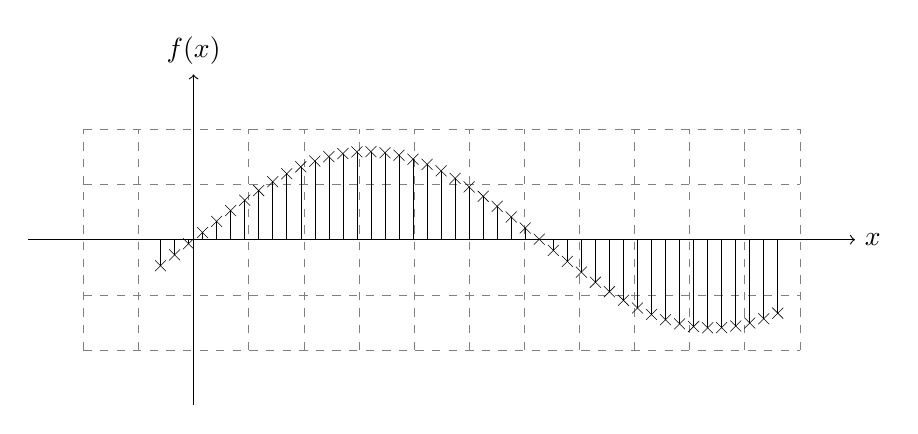
\begin{tikzpicture}[scale=1.4]
%grid
\draw[very thin,color=gray,step=.5cm,dashed] (-1,-1.0) grid (5.5,1);
\draw[->,color=black] (0,-1.5) -- (0,1.5)  node [above]{$f(x)$};
\draw[->,color=black] (-1.5,0) --  (6,0) node [right] {$x$};  
\draw[very thin,color=black,samples=45,domain=-0.3:5.3] 
plot[ycomb,thin,mark=x] (\x, { 0.8 * sin(\x r) });  
\end{tikzpicture}
	\end{center}
\end{figure}

\subsubsection{Samplefrequentie}

De samplefrequentie bepaalt het aantal samples per seconde en wordt uitgedrukt in Hertz ($Hz$). Bij het bepalen van de samplefrequentie is het van belang om rekening te houden met het \textit{bemonsteringstheorema van Nyquist-Shannon}. Deze stelling zegt dat de samplefrequentie minstens dubbel zo hoog moet zijn dan de maximumfrequentie van de te converteren informatie. Bij het gebruik van een lagere frequentie treedt er informatieverlies op. Deze stelling wordt in detail besproken in het originele artikel \cite{nyquist1928certain} van \citeauthor{nyquist1928certain}.

Het menselijk oor is in staat om geluiden te detecteren tussen 20Hz en 20kHz. Om informatieverlies bij het samplen van geluiden binnen dit bereik te voorkomen is het dus vereist om een minimale samplefrequentie te hanteren van $ 2 \times 20kHz $. De standaard samplefrequentie voor muziek is net iets hoger: $ 44.1kHz $.

De frequentie van de menselijke stem varieert tussen $ 30 Hz $ en $ 3000 Hz $. De minimale samplefrequentie voor het digitaliseren van een stemopname is dus $ 6kHz $. In de praktijk wordt meestal een minimum gehanteerd van $ 8kHz $.

\subsubsection{Bitdiepte}

De bitdiepte is het aantal bits waarmee elke gesamplede waarde wordt voorgesteld. Meestal wordt er gebruik gemaakt van 16 bit \textit{signed integers}.

De bitdiepte bepaald het dynamische bereik van audio. Dit is de verhouding tussen het stilst en luidst mogelijk weer te geven volume. Deze verhouding, uitgedrukt in decibel, kan worden berekend met volgende formule: 
\begin{equation}
DR = 20 \cdot \log_{10} \left(\frac{2^Q}{1}\right) = (6.02 \cdot Q) dB
\end{equation}

In deze formule staat DR voor het dynamische bereik en Q voor de bitdiepte. Volgens deze formule heeft 16 bit audio een theoretisch dynamische bereik van ongeveer 96 dB. De werkelijke waarde kan hier echter van afwijken door filters die zijn ingebouwd in audiosystemen.

Bovenstaande informatie is gebaseerd op artikel \cite{tarsosmanual2016}, introductievideo \cite{xiph2016} en boek \cite{fries2005digital}.

\section{Evaluatiecriteria}
\label{evaluatie-criteria}

Het te ontwikkelen systeem moet voldoen aan heel wat vereisten. In deze sectie zullen de vereisten eenduidig geformuleerd en besproken worden.  

\subsubsection{Realtime synchronisatie}

Een cruciale vereiste is dat de toepassing in \textit{realtime} moet kunnen werken. Concreet wil dit zeggen dat het tijdens het uitvoeren van het experiment mogelijk moet zijn om de huidige latencies van de streams op te vragen.

Het is moeilijk om het opvragen van deze gegevens echt in realtime mogelijk te maken. Veel algoritmes vereisen een bepaalde hoeveelheid aan data voordat de latency berekend kan worden. Daarom moeten de streams gebufferd worden, wat er toe leidt dat het systeem niet meer realtime is in de enge zin van het woord. Om een realtime systeem zo goed mogelijk te benaderen wordt een beperking opgelegd: een buffer met als maximumgrootte de hoeveelheid data verzameld in tien seconden. Deze tijd is de maximaal mogelijke achterstand ten opzichte van de realtime latency.

\subsubsection{Detecteren van gedropte samples}

De beperkte resources van een microcontroller kan voor problemen zorgen bij het verwerken van streams. Zo kan het gebeuren dat er gegevens van streams verloren gaan, in het vakjargon worden dit ook wel \textit{gedropte samples} genoemd. Bij de synchronisatie leidt dit probleem tot een plotse verhoging van de latency. Hoewel het onmogelijk is om de gedropte samples te reconstrueren is het wel gewenst dat de wijziging in latency gedetecteerd wordt en dat hiermee wordt rekening gehouden bij de verdere verwerking. De snelheid waarmee dit probleem gedetecteerd kan worden hangt eveneens af van de manier waarop er gebufferd wordt. Een detectie is mogelijk vanaf het moment dat de buffer voor meer dan de helft gevuld is met data gegenereerd na het gegevensverlies. Rekening houdend met het eerste criterium zou een wijziging van de latency binnen vijf seconden gedetecteerd moeten kunnen worden.

\subsubsection{Detecteren van drift}

Elke stream heeft een bepaalde samplefrequentie. Het is belangrijk dat de samplefrequentie gekend is om de gegevens correct en precies te kunnen verwerken. Het kan echter voorvallen dat de samplefrequentie bij de verwerking op microcontrollers minder nauwkeurig gekend is. Een stream waarbij de samplefrequentie $ 1Hz $ afwijkt van de theoretische waarde zal na 60 seconden een latency hebben opgebouwd van 60 samples. Bij een samplefrequentie van 8000 Hz komt dit overeen met 7,5 ms.\footnote{Berekening: $ 60 / 8000 Hz = 0.0075 s = 7.5 ms $} Dit probleem mag zeker niet worden verwaarloosd. 

\section{Bestaande methoden}
\label{bestaande-methoden}

Er bestaan verschillende methoden om datastreams te synchroniseren. Welke methode te verkiezen is hangt volledig af van de toepassing.

In deze sectie komen de belangrijkste methoden aan bod en zullen ze worden getoetst aan de eerder beschreven evaluatiecriteria. 

\subsection{Event-gebaseerde synchronisatie}

Deze methode wordt beschreven in \cite{bannach2009automatic, six2015multimodal} en is een eenvoudige, intuïtieve methode om synchronisatie van verschillende datastreams uit te voeren. De synchronisatie gebeurt aan de hand van markeringen die in de verschillende streams worden aangebracht. In audiostreams kan een kort en krachtig geluid een markering plaatsen. Een lichtflits kan dit realiseren in videostreams. De latency wordt bepaald door het verschil te berekenen tussen de tijdspositie van de markeringen in de streams. De synchronisatie kan vervolgens zowel manueel als softwarematig worden uitgevoerd.

Deze methode kent heel wat beperkingen. Zo vormt bij de synchronisatie van een groot aantal streams de schaalbaarheid een probleem. Ook wanneer er in een stream samples gedropt worden of er drift ontstaat, leidt dit tot foutieve synchronisatie. De methode kan deze twee problemen niet detecteren tot er opnieuw markeringen worden aangebracht en de streams gesynchroniseerd worden. Verder laten ook niet alle sensoren toe om markeringen aan te brengen: zo is de synchronisatie van een ECG onmogelijk met deze methode.

Het handmatig synchroniseren met behulp van deze methode blijkt derhalve in een realtime situatie niet mogelijk.  Wanneer de synchronisatie echter door software wordt uitgevoerd is deze methode wel in realtime bruikbaar. In dat geval moet er per tijdsinterval een markering worden aangebracht om de problemen veroorzaakt door drift en gedropte samples te overbruggen.

\subsection{Synchronisatie met een kloksignaal}

Artikel \cite{jaimovich2010synchronization} beschrijft een methode waarbij door een kloksignaal realtime streams van verschillende soorten toestellen worden gesynchroniseerd. Hiervoor gebruikt men standaard audio en video synchronisatieprotocollen. Elk toestel kan gebruik maken van verschillende samplefrequenties en communicatieprotocollen.

De methode gebruikt een \textit{master time code} signaal dat verstuurd wordt naar elk toestel. Dit laat het realtime analyseren van elke stream toe. Bij deze analyse kan vervolgens meteen de samplefrequentie en latency bepaald worden. 

Een groot nadeel van dit systeem is dat elk toestel een kloksignaal als input moet kunnen toelaten en verwerken. In het geval van de verwerking van videobeelden kan deze methode enkel gebruikt worden met zeer dure videocamera's waarbij de sluitertijd gecontroleerd kan worden. Bij goedkopere camera's (zoals's webcams) moet men op zoek gaan naar alternatieven. \cite{six2015multimodal}



\subsection{Dynamic timewarping}

Dynamic timewarping (DTW) is een techniek die gebruikt wordt voor het detecteren van gelijkenissen tussen twee tijdreeksen\footnote{Een tijdreeks is een sequentie van opeenvolgende datapunten over een continu tijdsinterval, waarbij de datapunten elk baar na telkens hetzelfde interval opvolgen.}. Aangezien een gedigitaliseerde audiostream een tijdreeks is kan deze techniek worden aangewend om de latency te bepalen tussen gelijkaardige opnames van het omgevingsgeluid. In de probleemschets (\ref{probleemschets}) is er uitgelegd hoe datastreams met behulp van het omgevingsgeluid gesynchroniseerd kunnen worden.

DTW is een algoritme dat op zoek gaat naar de meest optimale \textit{mapping} tussen twee tijdreeksen. Hierbij wordt gebruik gemaakt van een padkost. De padkost wordt bepaald door de manier waarop de tijdreeksen niet-lineair worden kromgetrokken ten opzichte van de tijdas\cite{salvador2007toward}. De minimale kost kan in kwadratische tijd berekend worden door gebruik te maken van dynamisch programmeren \cite{dixon2005live}. DTW is een veelgebruikte techniek in domeinen zoals spraakherkenning, bio-informatica, data-mining, etc \cite{ratanamahatana2004everything}.

Aangezien DTW het toelaat om tijdreeksen krom te trekken is het gewenst dat zowel het verleden als de toekomst van de streams voor het algoritme toegankelijk is. Een uitbreiding op dit algoritme beschreven in \cite{dixon2005live} laat toe één tijdreeks in realtime te streamen mits de andere stream op voorhand is gekend. Toch houdt deze uitbreiding geen oplossing in voor het gestelde probleem. Alle streams komen immers in realtime toe en we willen zo snel mogelijk de latency tussen de streams achterhalen.

Het bufferen van de binnenkomende streams en vervolgens het DTW algoritme uit te voeren op de buffers leek een mogelijke manier om dit probleem te omzeilen.

Of het algoritme na deze aanpassing voldoet aan onze vereisten diende een klein experiment uit te wijzen. De resultaten hiervan zijn te vinden in appendix \ref{appendix-a}: .

Het experiment toonde evenwel aan dat DTW niet bruikbaar is voor de realtime stream synchronisatie. De resultaten bleken niet nauwkeurig genoeg, zeker niet wanneer ook de performantie van het algoritme in beschouwing werd genomen.

\subsection{Accoustic fingerprinting}

Accoustic fingerprinting is een techniek die in staat is om gelijkenissen te vinden tussen verschillende audiofragmenten. Het is eveneens mogelijk om de latency tussen de audiofragmenten te bepalen. Net zoals bij DTW kan dit algoritme gebruikt worden om datastreams te synchroniseren met behulp van het omgevingsgeluid.

De techniek van accoustic fingerprinting extraheert en vergelijkt fingerprints van audiofragmenten. Een accoustic fingerprint bevat gecondenseerde informatie gebaseerd op typische eigenschappen van het audiofragment. De kracht van dit algoritme schuilt in haar snelheid en robuustheid. Het is immers uitzonderlijk bestand tegen achtergrondgeluiden en ruis. Door deze eigenschappen is het algoritme in staat om in enkele seconden een database met miljoenen fingerprints van audiofragmenten te doorzoeken. De bekendste toepassing van accoustic fingerprinting is de identificatie van liedjes op basis van een korte opname\footnote{Het grootste voorbeeld hiervan is de smartphone app Shazam. Deze app is de eerste toepassing dat gebruik maakte van dit algoritme.}.

Het is onder meer deze techniek die het IPEM gebruikt om de opgenomen audiostreams van experimenten te synchroniseren. In tegenstelling tot \textit{Shazam} wordt er niet op zoek gegaan naar matches in een database maar worden ze gezocht tussen de opgenomen audiofragmenten. Het uitgangspunt is immers dat er tussen de opnames gelijkenissen moeten gevonden kunnen worden.

Door haar snelheid en robuustheid lijkt dit algoritme te voldoen aan de vereisten om datastreams realtime te kunnen synchroniseren. Het is wel noodzakelijk dat de streams gebufferd worden alvorens het algoritme kan starten. Drift en gedropte samples kunnen gedetecteerd worden door het algoritme iteratief op korte gebufferde fragmenten uit te voeren. Na elke iteratie kan een eventuele wijziging worden opgemerkt. Zie \ref{accoustic-fingerprinting} voor een meer gedetailleerde bespreking van dit algoritme.

\subsection{Kruiscovariantie}

De laatste methode is net zoals de twee vorige methodes in staat om de latency tussen audiofragmenten te bepalen. Deze methode kan daarom ook aangewend worden om datastreams met behulp van opnames van het omgevingsgeluid te synchroniseren.

Kruiscovariantie (ook wel kruiscorrelatie genoemd) berekent de gelijkenis tussen twee audiofragmenten sample per sample en kent een getal toe aan de mate waarin de fragmenten overeenkomen. Door deze berekening voor elke verschuiving uit te voeren kan de latency tussen de fragmenten bepaald worden.

Deze methode is eveneens toepasbaar op realtime streams door gebruik te maken van buffering. Het iteratief uitvoeren van het algoritme op de opeenvolgende buffers zorgt ervoor dat gedropte samples en drift gedetecteerd kunnen worden.

In sectie \ref{kruiscovariantie} wordt deze materie verder in detail behandeld.

\section{Doel van deze masterproef}

Dit onderzoek wil drie zaken bereiken: 

\subsubsection{Selectie en optimalisatie van algoritmes}
Er wordt op zoek gegaan naar de algoritmes waarmee het probleem kan worden opgelost. Verder dienen de algoritmes en bijhorende parameters te worden geoptimaliseerd om in deze toepassing zo efficiënt mogelijk te presteren. Indien mogelijk zal er worden geprobeerd om de algoritmes waarvan er bij het IPEM al een implementatie beschikbaar is te hergebruiken.

Het beoogde doel is dat de algoritmes in staat zijn om audio opgenomen met een basic microfoon op een microcontroller te synchroniseren met een nauwkeurigheid van minstens één milliseconde.

\subsubsection{Ontwerp en implementatie van een softwarebibliotheek}
Het tweede doel van het onderzoek betreft het schrijven van een softwarebibliotheek. Deze bibliotheek zal gebruik maken van de geoptimaliseerde algoritmes om de audiostromen te synchroniseren. Deze bibliotheek moet vanuit andere software kunnen worden opgeroepen en gedetailleerde informatie teruggeven over de synchronisatie van de verschillende audiostreams.

\subsubsection{Ontwerp en implementatie van een gebruiksvriendelijke interface}

Uiteindelijk is het de bedoeling dat dit onderzoek resulteert in een gebruiksvriendelijke applicatie die toegankelijk is voor onderzoekers/musicologen zonder uitgebreide informatica kennis. De software moet in staat zijn om van verschillende binnenkomende datastromen (vergezeld met audiostream) te synchroniseren en op één of andere manier weg te schrijven naar een persistent medium.
